% 2012 年天津卷文科第 13 题：AB、AC 为圆的两条弦，过 B 的切线交 AC 延长线于 D，
% 过 C 作 BD 的平行线交圆于 E、交 AB 于 F。
% 来源 PDF：普通高考/2012/2012天津文.pdf，第 1 页（印面 777）第 2 栏。
% 重绘依据：按 AF=3、FB=1、EF=3/2 反算圆半径 R=sqrt(64/15)≈2.066，
%   A(-2,0.516)、B(2,0.516)、C(1.5,-1.420)、E(0.625,1.969)、D(2.667,-2.066)。
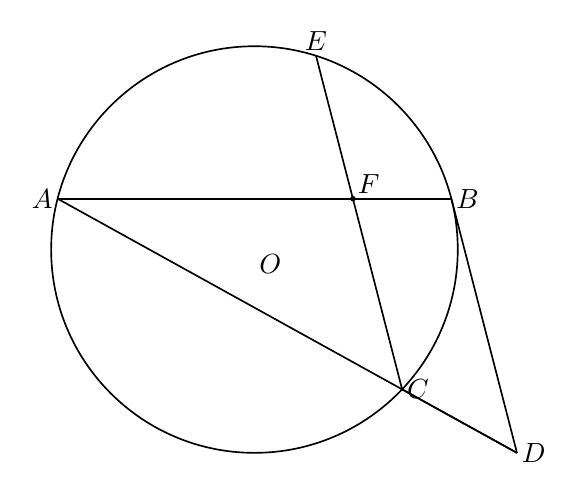
\begin{tikzpicture}[scale=1.25, semithick, every node/.style={inner sep=1.5pt}]
  \coordinate (O) at (0,0);
  \draw (O) circle (2.0656);
  \coordinate (A) at (-2,0.5164);
  \coordinate (B) at (2,0.5164);
  \coordinate (C) at (1.5,-1.4201);
  \coordinate (E) at (0.625,1.9688);
  \coordinate (F) at (1,0.5164);
  \coordinate (D) at (2.6667,-2.0656);
  \draw (A) -- (B);
  \draw (A) -- (D);
  \draw (C) -- (D);
  \draw (B) -- (D);
  \draw (C) -- (E);
  \fill (F) circle (0.8pt);
  \node[left] at (A) {$A$};
  \node[right] at (B) {$B$};
  \node[right] at (C) {$C$};
  \node[right] at (D) {$D$};
  \node[above] at (E) {$E$};
  \node[above right] at (F) {$F$};
  \node[below right] at (O) {$O$};
\end{tikzpicture}
